
\section{External Interface Requirements}
\label{s:External_interface_requirements}%

\subsection{User Interfaces}
\label{ss:User_interfaces}%

The CKB user interface will be a web page that will be accessed through a web browser. The web page will be designed to be simple and easy to use with the support for multiple screen sizes and devices.

\subsection{Hardware Interfaces}
\label{ss:Hardware_interfaces}%

The platform requires a computer with a web browser and an internet connection to access the CKB web page. 

\subsection{Software Interfaces}
\label{ss:Software_interfaces}%

CKB will be using some software interfaces both from external systems and internal implemented ones in order to provide the services. The interfaces used are listed below:
\begin{itemize}
  \item \textbf{Github API:} CKB will use Github as source control system for the projects. The Github API will be used to create the repositories for each team in the battle and share it with the team members.
  \item \textbf{Static Analyzer:} CKB will use a static analysis tool to analyze the code of each team after every new commit and will use the result of the analysis to assign points to each team. The purpose of this interface is to give the possibility to the system to configure the analyzer as the educator needs, in terms of test cases, languages supported and other parameters.
  \item \textbf{Results API: } The \textit{SA\_Server} will use this API to send the results of the analysis to the main server.
  \item \textbf{Github Actions: } Github Actions will notify the system when a participant has pushed a new commit to its repository. The \textit{SA\_Server} will be listening to this notifications and will trigger the analysis of the source code.
\end{itemize}

\subsection{Communication Interfaces}
\label{ss:Communication_interfaces}%

All the communication between CKB, the external interfaces and the user will be done using HTTPS protocol.

\subsection{List of Requirements}
\label{ss:List_of_Requirements}%
\begin{center}
  \begin{longtable}{|p{3cm}|p{0.8\linewidth}|}
        \hline
        \textbf{Requirement} & \textbf{Description} \\
        \hline
        R1 & CKB shall allow an unregistered user to create an account \\
        \hline
        R2 & CKB shall allow users to log in \\
        \hline
        R3 & CKB shall allow ST to connect their Github account \\
        \hline
        R4 & CKB shall allow ED to create competition \\
        \hline
        R5 & CKB shall allow ED to create battle within a competition \\
        \hline
        R6 & CKB shall allow ED to invite other EDs to create battles in a competition \\
        \hline
        R7 & CKB shall allow ED to upload the code kata \\
        \hline
        R8 & CKB shall allow ED to set a registration deadline to the battle \\
        \hline
        R9 & CKB shall allow ED to set a minimum number of STs per group in a battle \\
        \hline
        R10 & CKB shall allow ED to set the maximum number of STs per group in a battle \\
        \hline
        R11 & CKB shall allow ED to set a final submission deadline \\
        \hline
        R12 & CKB shall allow ED to set how to perform static analysis \\
        \hline
        R13 & CKB shall allow ST to subscribe to a competition \\
        \hline
        R14 & CKB shall send notifications about a new competition to ST \\
        \hline
        R15 & CKB shall send notification about battle created within a competition ST are subscribed in \\
        \hline
        R16 & CKB shall allow ST to join a battle on his own \\
        \hline
        R17 & CKB shall allow ST to invite other ST in a T for a battle \\
        \hline
        R18 & CKB shall create a GitHub repository containing the code kata \\
        \hline
        R19 & CKB shall send the Github repository link to ST member of a T competing in the battle \\
        \hline
        R20 & CKB shall supply API to call with Github actions \\
        \hline
        R21 & CKB shall be able to pull sources from GitHub \\
        \hline
        R22 & CKB shall be able to send the ST source code to the correct SAT \\
        \hline
        R23 & CKB shall be able to receive the evaluation given by SAT on a source code \\
        \hline
        R24 & CKB shall be able to run tests on code \\
        \hline
        R25 & CKB shall evaluate the code in terms of test cases passed \\
        \hline
        R26 & CKB shall evaluate the code in terms of timeliness \\
        \hline
        R27 & CKB shall allow ED to assign a score to codes \\
        \hline
        R28 & CKB shall update the score of a T (as soon as new push actions are performed) \\
        \hline
        R29 & CKB shall allow ED to go through sources produced by Ts \\
        \hline
        R30 & CKB shall notify ST when final battle ranks are available \\
        \hline
        R31 & CKB shall update the personal competition score of a ST at the end of each battle \\
        \hline
        R32 & CKB shall create a rank with students' performances in a competition \\
        \hline
        R33 & CKB shall allow ST to see all ST’s rank in battle where is enrolled \\
        \hline
        R34 & CKB shall allow ED to see all ST’s ranks in the battle that he/she manages \\
        \hline
        R35 & CKB shall allow EDs and STs to see all ST’s rank in competitions \\
        \hline
        R36 & CKB shall allow ST to see the list of ongoing competitions \\
        \hline
        R37 & CKB shall allow ED to close a competition \\
        \hline
        R38 & CKB shall allow ED to define badges in the context of a competition \\
        \hline
        R39 & CKB shall assign badges to students at the end of the competition \\
        \hline
        R40 & CKB shall allow ED to define new rules for badges \\
        \hline
        R41 & CKB shall allow ED to define new variables for badges \\
        \hline
        R42 & CKB shall allow users to visualize badges obtained by a ST \\
        \hline
        R43 & CKB shall allow users to visualize a ST profile \\
        \hline
        R44 & CKB shall allow ST to join a T for which is invited \\
        \hline
        R45 & CKB shall allow ST to join a public T \\
        \hline
        R46 & CKB shall allow ST to create a T \\
        \hline
        R47 & CKB shall allow ST to set a T to public or private \\
        \hline
        R48 & CKB can distinguish between an ED user and a ST user \\
        \hline
        R49 & CKB shall not allow ST/ED to see the rankings of battles in competitions they are not involved in \\
        \hline
        R50 & CKB shall have the environments for all the programming language it supports \\
        \hline
        R51 & CKB shall allow ED to close a battle they manage \\
        \hline

  \end{longtable}
\end{center}


\subsection{Mapping on Goals}
\label{ss:Mapping_requirements}%

\begin{table}[H]
  \begin{tabular}{|l|p{9cm}|p{5cm}| }
    \hline
    \textbf{Goal} & \textbf{Requirements} & \textbf{Domain Assumptions}      \\
    \hline
    G1 & R1 R2 R4 R6 R37 R38 R40 R41 R48 R49 & DA4 DA13 DA15 DA16 \\
    \hline
    G2 & R1 R2 R4 R5 R6 R7 R8 R9 R10 R11 R12 R34 R48 R49 R51 & DA5 DA6 DA7 DA13 \\
    \hline
    G3 & R1 R2 R3 R13 R14 R15 R30 R31 R33 R35 R36 R48 R49 & DA1 DA2 DA3 DA4 DA12 \\
    \hline
    G4 & R1 R2 R13 R15 R16 R17 R44 R45 R46 R47 R48 & DA1 DA11 DA12 \\
    \hline
    G5 & R1 R2 R13 R14 R15 R17 R30 R48 & DA1 DA11 DA12 \\
    \hline
    G6 & R18 R19 R20 & DA9 \\
    \hline
    G7 & R2 R3 R19 R20 R21 & DA1 DA2 DA3 DA4 \\
    \hline
    G8 & R21 R22 R23 R24 R25 R26 R27 R28 R29 R31 R32 R50 & DA5 DA6 DA7 DA8 DA10 DA13 DA14 \\
    \hline
    G9 & R1 R2 R13 R15 R29 R30 R31 R32 R34 R33 R35 R49 & DA1 DA6 DA12 DA13 \\
    \hline
    G10 & R38 R39 R40 R41 R42 R48 & DA16 \\
    \hline
    G11 & R1 R2 R42 R43 & DA1 DA6 DA12 DA13 DA17 \\
    \hline
  \end{tabular}
  \caption{Mapping between goals, requirements, and domain assumptions}
  \label{tab:mapping}
\end{table}

  \begin{table}[H]
    \begin{tabular}{|l|p{12cm}| }
      \hline
      \textbf{G1} & \textbf{Enable ED to manage competitions}      \\
      \hline
      R1 & CKB shall allow an unregistered user to create an account \\
      \hline
      R2 & CKB shall allow users to log in \\
      \hline
      R4 & CKB shall allow ED to create competition \\
      \hline
      R6 & CKB shall allow ED to invite other EDs to create battles in a competition \\
      \hline
      R37 & CKB shall allow ED to close a competition \\
      \hline
      R38 & CKB shall allow ED to define badges in the context of a competition \\
      \hline
      R40 & CKB shall allow ED to define new rules for badges \\
      \hline
      R41 & CKB shall allow ED to define new variables for badges \\
      \hline
      R48 & CKB can distinguish between an ED user and a ST user \\
      \hline
      R49 & CKB shall not allow ST/ED to see the rankings of battles in competitions they are not involved in \\
      \hline
      DA4 & ST knows how to use Git \\
      \hline
      DA13 & ED has an internet connection \\
      \hline
      DA15 & ED knows the email of the other EDs he wants to invite to manage a competition \\
      \hline
      DA16 & ED writes the correct badge’ rules \\
      \hline
    \end{tabular}
    \caption{Specific mapping on G1}
    \label{tab:mappingG1}
  \end{table}

  \begin{longtable}{|l|p{12cm}| }
    \hline
    \textbf{G2} & \textbf{Enable ED to manage Code Battles within Competitions}      \\
    \hline
    R1 & CKB shall allow an unregistered user to create an account \\
    \hline
    R2 & CKB shall allow users to log in \\
    \hline
    R4 & CKB shall allow ED to create competition \\
    \hline
    R5 & CKB shall allow ED to create battle within a competition \\
    \hline
    R6 & CKB shall allow ED to invite other EDs to create battles in a competition \\
    \hline
    R7 & CKB shall allow ED to upload the code kata \\
    \hline
    R8 & CKB shall allow ED to set a registration deadline to the battle \\
    \hline
    R9 & CKB shall allow ED to set a minimum number of STs per group in a battle \\
    \hline
    R10 & CKB shall allow ED to set the maximum number of STs per group in a battle \\
    \hline
    R11 & CKB shall allow ED to set a final submission deadline \\
    \hline
    R12 & CKB shall allow ED to set how to perform static analysis \\
    \hline
    R34 & CKB shall allow ED to see all ST’s ranks in the battle that he/she manages \\
    \hline
    R48 & CKB can distinguish between an ED user and a ST user \\
    \hline
    R49 & CKB shall not allow ST/ED to see the rankings of battles in competitions they are not involved in \\
    \hline
    R51 & CKB shall allow ED to close a battle they manage \\
    \hline
    DA5 & ED knows how to use Git \\
    \hline
    DA6 & ED owns a device able to connect to the internet \\
    \hline
    DA7 & ED writes correct tests \\
    \hline
    DA13 & ED has an internet connection \\
    \hline

    \caption{Specific mapping on G2}
    \label{tab:mappingG2}
  \end{longtable}

  \pagebreak 


  \begin{longtable}{|l|p{12cm}| }
    \hline
    \textbf{G3} & \textbf{Enable ST to participate in a Competition}      \\
    \hline
    R1 & CKB shall allow an unregistered user to create an account \\
    \hline
    R2 & CKB shall allow users to log in \\
    \hline
    R3 & CKB shall allow ST to connect their Github account \\
    \hline
    R13 & CKB shall allow ST to subscribe to a competition \\
    \hline
    R14 & CKB shall send notifications about a new competition to ST \\
    \hline
    R15 & CKB shall send notification about battle created within a competition ST is subscribed in \\
    \hline
    R30 & CKB shall notify ST when final battle ranks are available \\
    \hline
    R31 & CKB shall update the personal competition score of a ST at the end of each battle \\
    \hline
    R33 & CKB shall allow ST to see all ST’s rank in a battle where is enrolled \\
    \hline
    R35 & CKB shall allow EDs and STs to see all ST’s rank in competitions \\
    \hline
    R36 & CKB shall allow ST to see the list of ongoing competitions \\
    \hline
    R48 & CKB can distinguish between an ED user and a ST user \\
    \hline
    R49 & CKB shall not allow ST/ED to see the rankings of battles in competitions they are not involved in \\
    \hline
    DA1 & ST owns a device able to connect to the internet \\
    \hline
    DA2 & ST owns a GitHub account \\
    \hline
    DA3 & ST has installed Git on his computer \\
    \hline
    DA4 & ST knows how to use Git \\
    \hline
    DA12 & ST has an internet connection \\
    \hline

    \caption{Specific mapping on G3}
    \label{tab:mappingG3}
  \end{longtable}

  \begin{longtable}{|l|p{12cm}|}
    \hline
    \textbf{G4} & \textbf{Enable ST to be part of a team within a battle}      \\
    \hline
    R1 & CKB shall allow an unregistered user to create an account \\
    \hline
    R2 & CKB shall allow users to log in \\
    \hline
    R13 & CKB shall allow ST to subscribe to a competition \\
    \hline
    R15 & CKB shall send notification about battle created within a competition ST is subscribed in \\
    \hline
    R16 & CKB shall allow ST to join a battle on his own \\
    \hline
    R17 & CKB shall allow ST to invite other ST in a T for a battle \\
    \hline
    R44 & CKB shall allow ST to join a T for which is invited \\
    \hline
    R45 & CKB shall allow ST to join a public T \\
    \hline
    R46 & CKB shall allow ST to create a T \\
    \hline
    R47 & CKB shall allow ST to set a T to public or private \\
    \hline
    R48 & CKB can distinguish between an ED user and a ST user \\
    \hline
    DA1 & ST owns a device able to connect to the internet \\
    \hline
    DA11 & ST knows the usernames of other STs they want to invite to a T \\
    \hline
    DA12 & ST has an internet connection \\
    \hline

    \caption{Specific mapping on G4}
    \label{tab:mappingG4}
  \end{longtable}

  \begin{longtable}{|l|p{12cm}|}
    \hline
    \textbf{G5} & \textbf{Send Notifications to STs}      \\
    \hline
    R1 & CKB shall allow an unregistered user to create an account \\
    \hline
    R2 & CKB shall allow users to log in \\
    \hline
    R13 & CKB shall allow ST to subscribe to a competition \\
    \hline
    R14 & CKB shall send notifications about a new competition to ST \\
    \hline
    R15 & CKB shall send notification about battle created within a competition ST is subscribed in \\
    \hline
    R17 & CKB shall allow ST to invite other ST in a T for a battle \\
    \hline
    R30 & CKB shall notify ST when final battle ranks are available \\
    \hline
    R48 & CKB can distinguish between an ED user and a ST user \\
    \hline
    DA1 & ST owns a device able to connect to the internet \\
    \hline
    DA11 & ST knows the usernames of other STs they want to invite to a T \\
    \hline
    DA12 & ST has an internet connection \\
    \hline

    \caption{Specific mapping on G5}
    \label{tab:mappingG5}
  \end{longtable}

  \begin{longtable}{|l|p{12cm}|}
    \hline
    \textbf{G6} & \textbf{Automatically Create GitHub Repositories for Every Battle in a Competition}      \\
    \hline
    R18 & CKB shall create a GitHub repository containing the code kata \\
    \hline
    R19 & CKB shall send the Github repository link to ST member of a T competing in the battle \\
    \hline
    R20 & CKB shall supply API to call with Github actions \\
    \hline
    DA9 & GitHub permits automatic push to a repository \\
    \hline

    \caption{Specific mapping on G6}
    \label{tab:mappingG6}
  \end{longtable}
  
  \begin{longtable}{|l|p{12cm}|}
    \hline
    \textbf{G7} & \textbf{Synchronize the Submission of Each Candidate with Their GitHub Repository}      \\
    \hline
    R2 & CKB shall allow users to log in \\
    \hline
    R3 & CKB shall allow ST to connect their Github account \\
    \hline
    R19 & CKB shall send the Github repository link to ST member of a T competing in the competition \\
    \hline
    R20 & CKB shall supply API to call with Github actions \\
    \hline
    R21 & CKB shall be able to pull sources from GitHub \\
    \hline
    DA1 & ST owns a device able to connect to the internet \\
    \hline
    DA2 & ST owns a GitHub account \\
    \hline
    DA3 & ST has installed Git on his computer \\
    \hline
    DA4 & ST knows how to use Git \\
    \hline

    \caption{Specific mapping on G7}
    \label{tab:mappingG7}
  \end{longtable}


  \begin{longtable}{|l|p{12cm}|}
    \hline
    \textbf{G8} & \textbf{CKB Provides an evaluation of the code submitted}      \\
    \hline
    R21 & CKB shall be able to pull sources from GitHub \\
    \hline
    R22 & CKB shall be able to send the ST source code to the correct SAT \\
    \hline
    R23 & CKB shall be able to receive the evaluation given by SAT on a source code \\
    \hline
    R24 & CKB shall be able to run tests on code \\
    \hline
    R25 & CKB shall evaluate the code in terms of test cases passed \\
    \hline
    R26 & CKB shall evaluate the code in terms of timeliness \\
    \hline
    R27 & CKB shall allow ED to assign a score to codes \\
    \hline
    R28 & CKB shall update the score of a T (as soon as new push actions are performed) \\
    \hline
    R29 & CKB shall allow ED to go through sources produced by Ts \\
    \hline
    R31 & CKB shall update the personal competition score of a ST at the end of each battle \\
    \hline
    R32 & CKB shall create a rank with students' performances in a competition \\
    \hline
    R50 & CKB shall have the environments for all the programming language it supports \\
    \hline
    DA5 & ED knows how to use Git \\
    \hline
    DA6 & ED owns a device able to connect to the internet \\
    \hline
    DA7 & ED writes correct tests \\
    \hline
    DA8 & ED correctly evaluates the final source code of a T \\
    \hline
    DA10 & Github permits automatical pull from a repository \\
    \hline
    DA13 & ED has an internet connection \\
    \hline
    DA14 & ST writes code only with languages that are treatable by the platform \\
    \hline

    \caption{Specific mapping on G8}
    \label{tab:mappingG8}
  \end{longtable}

  \begin{longtable}{|l|p{12cm}|}
    \hline
    \textbf{G9} & \textbf{Allow users to View Rankings in both battles and competitions}      \\
    \hline
    R1 & CKB shall allow an unregistered user to create an account \\
    \hline
    R2 & CKB shall allow users to log in \\
    \hline
    R13 & CKB shall allow ST to subscribe to a competition \\
    \hline
    R15 & CKB shall send notification about battle created within a competition ST is subscribed in \\
    \hline
    R29 & CKB shall allow ED to go through sources produced by Ts \\
    \hline
    R30 & CKB shall notify ST when final battle ranks are available \\
    \hline
    R31 & CKB shall update the personal competition score of a ST at the end of each battle \\
    \hline
    R32 & CKB shall create a rank with students' performances in a competition \\
    \hline
    R33 & CKB shall allow ST to see all ST’s rank in a battle where is enrolled \\
    \hline
    R34 & CKB shall allow ED to see all ST’s ranks in the battle that he/she manages \\
    \hline
    R35 & CKB shall allow EDs and STs to see all ST’s rank in competitions \\
    \hline
    R49 & CKB shall not allow ST/ED to see the rankings of battles in competitions they are not involved in \\
    \hline
    DA1 & ST owns a device able to connect to the internet \\
    \hline
    DA6 & ED owns a device able to connect to the internet \\
    \hline
    DA12 & ST has an internet connection \\
    \hline
    DA13 & ED has an internet connection \\ 
    \hline

    \caption{Specific mapping on G9}
    \label{tab:mappingG9}
  \end{longtable}

  \begin{longtable}{|l|p{12cm}|}
    \hline
    \textbf{G10} & \textbf{Allow to assign badges to the students}      \\
    \hline
    R38 & CKB shall allow ED to define badges in the context of a competition \\
    \hline
    R39 & CKB shall assign badges to students at the end of the competition \\
    \hline
    R40 & CKB shall allow ED to define new rules for badges \\
    \hline
    R41 & CKB shall allow ED to define new variables for badges \\
    \hline
    R42 & CKB shall allow users to visualize badges obtained by a ST \\
    \hline
    R48 & CKB can distinguish between an ED user and a ST user \\
    \hline
    DA16 & ED writes the correct badge’ rules \\
    \hline

    \caption{Specific mapping on G10}
    \label{tab:mappingG10}
  \end{longtable}

  \begin{longtable}{|l|p{12cm}| }
    \hline
    \textbf{G11} & \textbf{Allow users to visualize ST profiles}      \\
    \hline
    R1 & CKB shall allow an unregistered user to create an account \\
    \hline
    R2 & CKB shall allow users to log in \\
    \hline
    R42 & CKB shall allow users to visualize badges obtained by a ST \\
    \hline
    R43 & CKB shall allow users to visualize a ST profile \\
    \hline
    DA1 & ST owns a device able to connect to the internet \\
    \hline
    DA6 & ED owns a device able to connect to the internet \\
    \hline
    DA12 & ST has an internet connection \\
    \hline
    DA13 & ED has an internet connection \\
    \hline
    DA17 & User knows the username of the STs' profile they want to visualize \\
    \hline
    \caption{Specific mapping on G11}
    \label{tab:mappingG11}
  \end{longtable}

\pagebreak

\subsection{Use Cases}
\label{ss:Use_cases}%

\subsubsection*{Use case diagram}
Here you can find the use case diagram of the platform. 
\begin{center}
  \begin{figure} [H]
    \begin{center}
        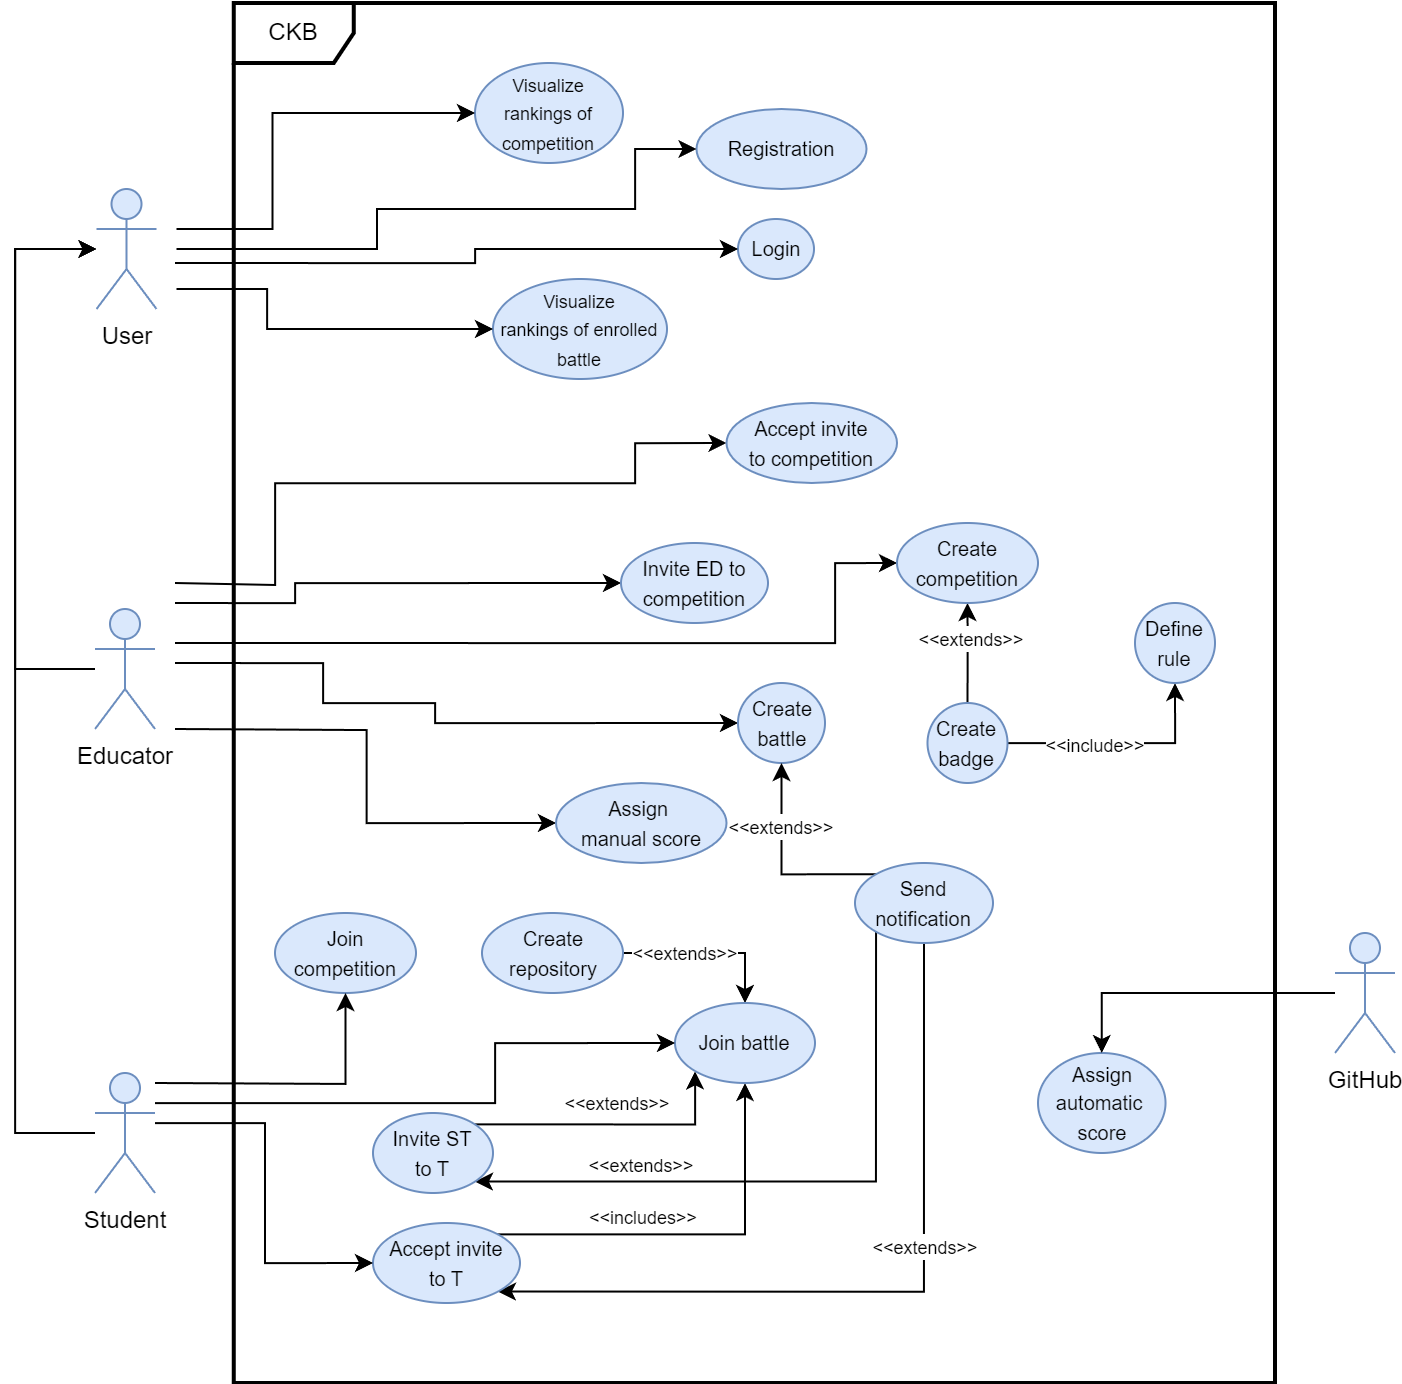
\includegraphics[width=\textwidth,height=\textheight,keepaspectratio]{Images/RASD_UseCaseDiagram.png}
        \caption{Use case diagram of the platform.}
        \label{fig: UseCaseDiagram}
    \end{center}
  \end{figure}
\end{center}

For simplicity we decided not to include all the \textit{<<include>>} relationship related to the \textbf{\textit{Login}} use case, since  almost every use case requires the user to be logged in, this was to explain that it was not forgotten.

\subsubsection*{UC1: Unregistered ST creates an account}
\begin{center}
  \begin{longtable}{l|p{0.75\linewidth}}
    \hline
    Actor & Unregistered ST \\
    \hline
    Entry conditions & The ST isn’t already registered in the \verb|CKB| platform and he clicks on the sign-up button \\
    \hline
    Event Flow & 1.\ CKB asks the ST to insert the personal information (i.e. name, surname, nickname, e-mail and password) \\
    & 2.\ The ST fills out the form with the requested information and accepts the “Terms \& Conditions” and “Privacy Policy” \\
    & 3.\ CKB validate the inserted information \\
    & 4.\ CKB sends an account activation link to the email inserted by the ST \\
    & 5.\ ST clicks on the link received in the email \\
    & 6.\ CKB confirms the account creation  \\
    \hline
    Exit condition & The ST account is created \\
    \hline
    Exceptions & 3.1 CKB isn’t able to validate the information inserted (i.e. duplicate email, duplicate username and wrong email address \\
    & 5.1 The link is expired \\ \\
    & In all the cases the ST is notified with an error message\\
    \hline
    \caption{ST signs up case.}
    \label{tab: ST_signs_up}
  \end{longtable}

  \begin{figure} [H]
    \begin{center}
        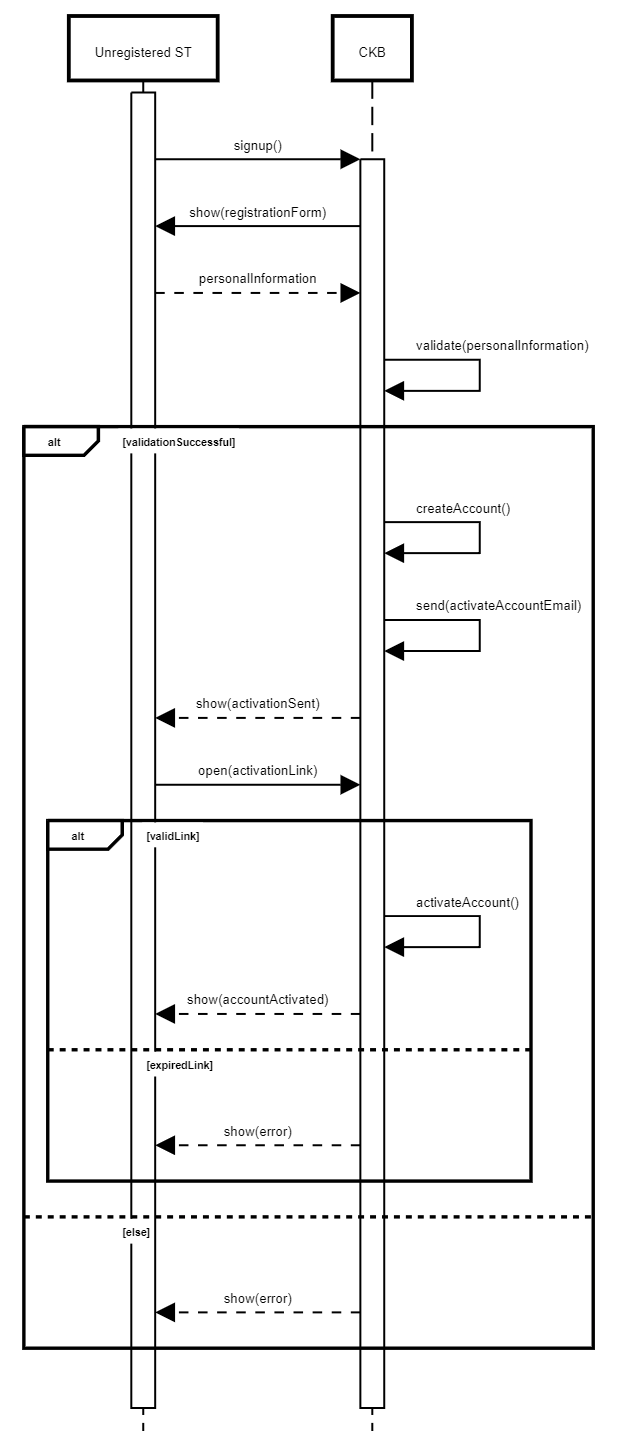
\includegraphics[width=\textwidth,height=\textheight,keepaspectratio]{Images/SequenceDiagrams/UC1.png}
        \caption{UC1 sequence diagram.}
        \label{fig: UC1_sequence_diagram}
    \end{center}
  \end{figure}
\end{center}

\subsubsection*{UC2: Unregistered ED creates an account}
\begin{center}
  \begin{longtable}{l|p{0.75\linewidth}}
    \hline
    Actor & Unregistered ED \\
    \hline
    Entry conditions & The ED isn’t already registered in the \verb|CKB| platform and he clicks on the sign-up button \\
    \hline
    Event Flow & 1.\ CKB asks the ED to insert the personal information (i.e. name, surname, nickname, e-mail and password) \\
    & 2.\ The ED fills out the form with the requested information and accepts the “Terms \& Conditions” and “Privacy Policy” \\
    & 3.\ CKB validate the inserted information \\
    & 4.\ CKB asks the ED to insert the information about the institution (i.e. name, address, city, country, website) \\
    & 5.\ The ED fills out the form with the requested information \\
    & 6.\ CKB validate the information about the institute \\
    & 7.\ CKB sends an account activation link to the email inserted by the ED \\
    & 8.\ ED clicks on the link received in the email \\
    & 9.\ CKB confirms the account creation  \\
    \hline
    Exit condition & The ED account is created \\
    \hline
    Exceptions & 3.1 CKB isn’t able to validate the information inserted (i.e. duplicate email, duplicate username and wrong email address \\
    & 6.1 CKB isn’t able to validate the information about the institute \\
    & 8.1 The link is expired \\ \\
    & In all the cases the ST is notified with an error message\\
    \hline
    \caption{ED signs up case.}
    \label{tab: ED_signs_up}
  \end{longtable}

  \begin{figure} [H]
    \begin{center}
        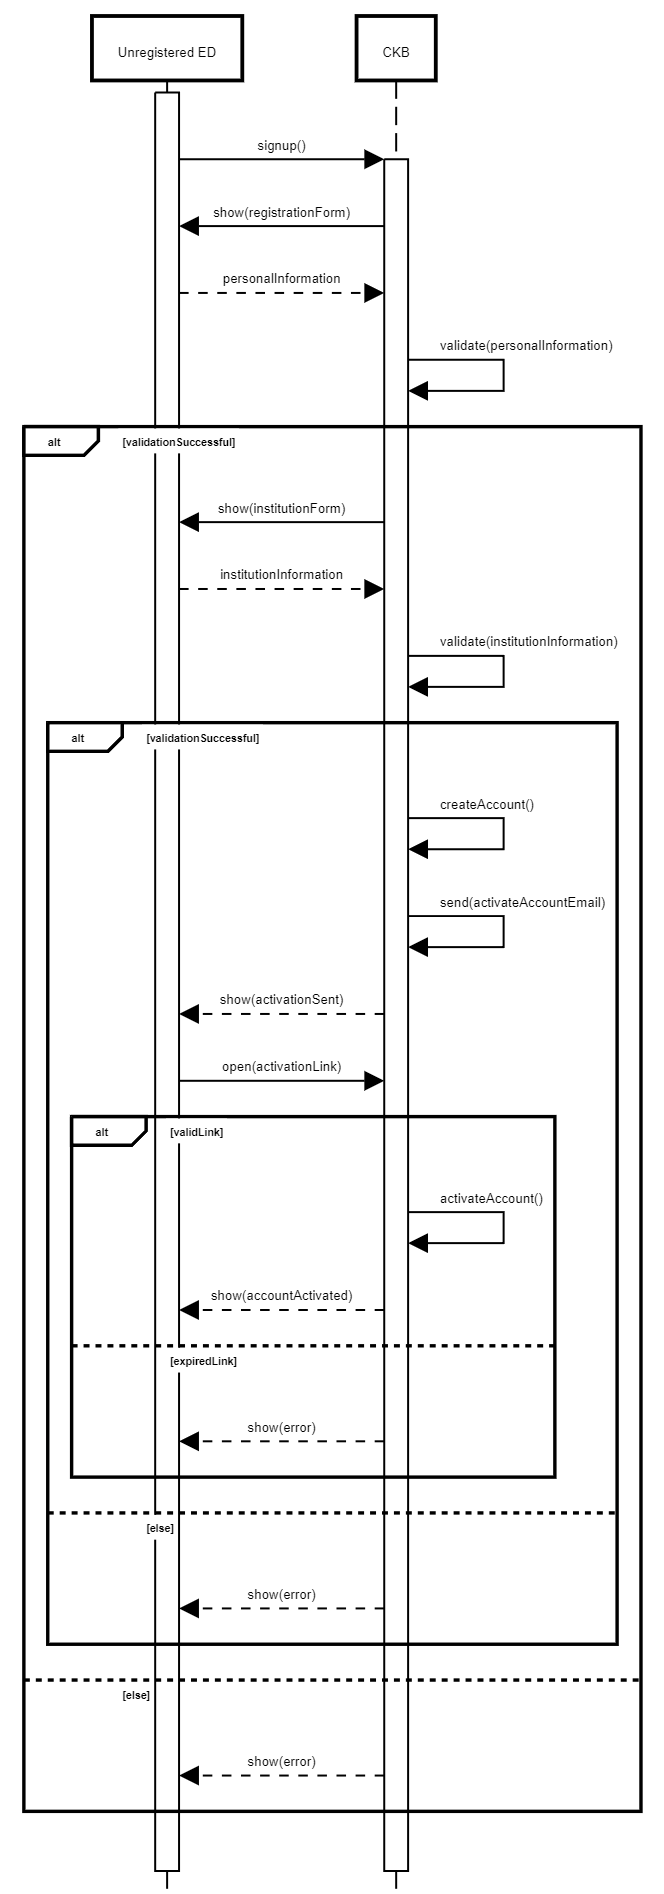
\includegraphics[width=\textwidth,height=\textheight,keepaspectratio]{Images/SequenceDiagrams/UC2.png}
        \caption{UC2 sequence diagram.}
        \label{fig: UC2_sequence_diagram}
    \end{center}
  \end{figure}
\end{center}

\subsubsection*{UC3: ST or ED logs in}
\begin{center}
  \begin{longtable}{l|p{0.75\linewidth}}
    \hline
    Actor & Registered ST \\
    & Registered ED \\
    \hline
    Entry conditions & The ED isn already registered in the \verb|CKB| platform \\
    \hline
    Event Flow & 1.\ The user clicks on the login button \\
    & 2.\ CKB asks for the username and the password \\
    & 3.\ The user inserts the username and the password \\
    & 4.\ CKB validates the information \\
    & 5.\ CKB redirects the user to the home page \\
    \hline
    Exit condition & The user is logged in \\
    \hline
    Exceptions & 4.1 The username or the password are wrong \\ \\
    & In this case the user is notified with an error message \\
    \hline
    \caption{ST or ED logs in.}
    \label{tab: ST_or_ED_logs_in}
  \end{longtable}

  \begin{figure} [H]
    \begin{center}
        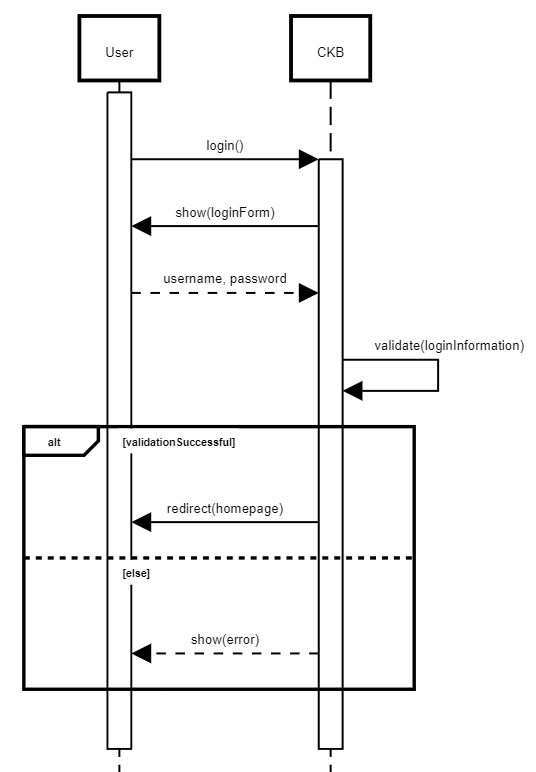
\includegraphics[width=0.65\textwidth,height=\textheight,keepaspectratio]{Images/SequenceDiagrams/UC3.png}
        \caption{UC3 sequence diagram.}
        \label{fig: UC3_sequence_diagram}
    \end{center}
  \end{figure}
\end{center}

\subsubsection*{UC4: ED creates a new competition}
\begin{center}
  \begin{longtable}{l|p{0.75\linewidth}}
    \hline
    Actor & Registered ED \\
    \hline
    Entry conditions & The ED is already registered and logged in  \\
    & The ED clicks on the “Create Competition” button \\
    \hline
    Event Flow & 1.\ CKB asks for a name for the competition \\
    & 2.\ The ED inserts the name \\
    & 3.\ CKB checks if the name is available \\
    & 4.\ CKB asks for the information of the competition (i.e. description, start date, end date, programming languages allowed) \\
    & 5.\ CKB validates the information \\
    & 6.\ CKB creates the competition \\
    \hline
    Exit condition & The competition is correctly created \\
    \hline
    Exceptions & 3.1 The name is already used by another competition \\
    & 5.1 CKB isn’t able to validate the information \\ \\
    & In the first case the ED is notified with an error message and the flow restarts from the step 1 \\
    & In the other case the ED is notified with an error message \\
    \hline
    \caption{ED creates a competiton.}
    \label{tab: ED_create_competition}
  \end{longtable}

  \begin{figure} [H]
    \begin{center}
        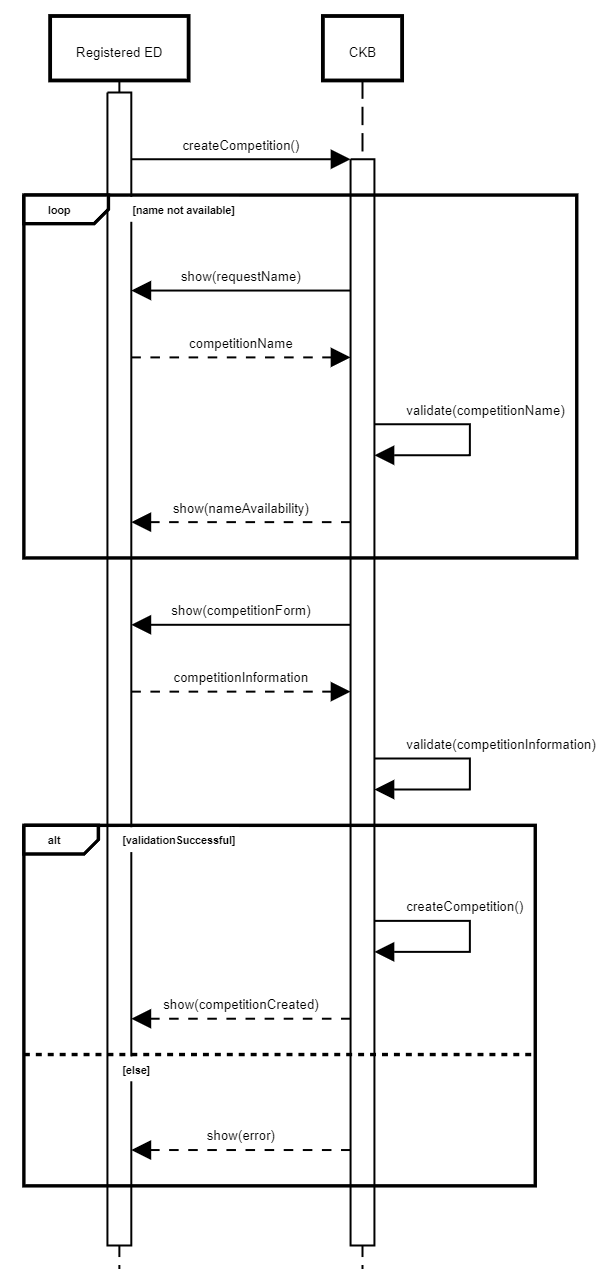
\includegraphics[width=\textwidth,height=\textheight,keepaspectratio]{Images/SequenceDiagrams/UC4.png}
        \caption{UC4 sequence diagram.}
        \label{fig: UC4_sequence_diagram}
    \end{center}
  \end{figure}
\end{center}

\subsubsection*{UC5: ST joins a competition}
\begin{center}
  \begin{longtable}{l|p{0.75\linewidth}}
    \hline
    Actor & Registered ST \\
    \hline
    Entry conditions & The ST is already registered and logged in  \\
    \hline
    Event Flow & 1.\ CKB shows the list of the available competitions \\
    & 2.\ The ST selects the competition \\
    & 3.\ CKB shows the information about the competition \\
    & 4.\ The ST clicks on the “Join” button \\
    & 5.\ CKB adds the ST to the competition \\
    & 6.\ ST can now see the competition in the “My Competitions” section \\
    \hline
    Exit condition & The ST has joined the competition \\
    \hline
    Exceptions & 2.1 There are no competitions available \\ \\
    & In this case the ST visualizes a message that there are no competition available \\ \\
    \hline
    \caption{ST joins a competition.}
    \label{tab: ST_join_competition}
  \end{longtable}

  \begin{figure} [H]
    \begin{center}
        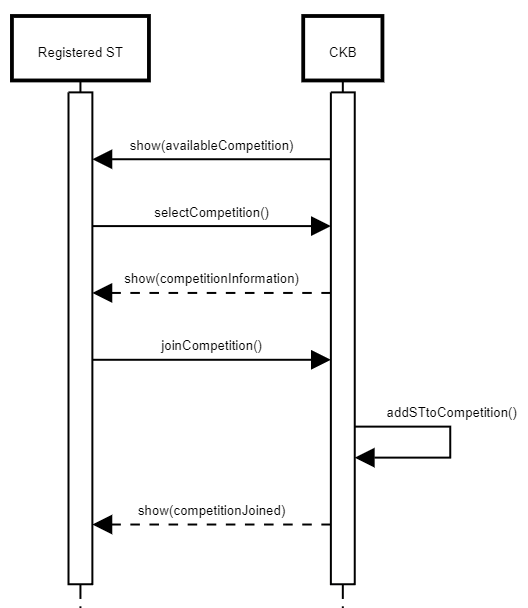
\includegraphics[width=0.65\textwidth,height=\textheight,keepaspectratio]{Images/SequenceDiagrams/UC5.png}
        \caption{UC5 sequence diagram.}
        \label{fig: UC5_sequence_diagram}
    \end{center}
  \end{figure}
\end{center}

\subsubsection*{UC6: ED creates a new battle inside a competition}
\begin{center}
  \begin{longtable}{l|p{0.75\linewidth}}
    \hline
    Actor & Registered ED \\
    \hline
    Entry conditions & The ED is already registered and logged in  \\
    & The ED is the creator or a collaborator of the competition \\
    & The ED is in the competition page \\
    & The ED clicks on the “Create Battle” button \\
    \hline
    Event Flow & 1.\ CKB asks for a name for the battle \\
    & 2.\ CKB checks if the name is not already used for another battle inside the competition \\
    & 3.\ CKB asks for the information of the battle (i.e. description, start date, end date, programming languages allowed, number of teams, number of members per team) \\
    & 4.\ ED inserts the information \\
    & 5.\ CKB asks for the configuration of the static analyzer \\
    & 6.\ CKB asks to upload the test cases and the solution \\
    & 7.\ ED uploads the files and insert all the information requested \\
    & 8.\ CKB validates the information \\
    & 9.\ CKB creates the battle \\
    \hline
    Exit condition & The battle is created correctly \\
    \hline
    Exceptions & 6.1 The upload of the files fails \\
    & 7.1 CKB isn’t able to validate the information \\ \\
    & In all the cases the ED is notified with an error message \\
    \hline
    \caption{ED creates a battle inside a competition.}
    \label{tab: ED_create_battle}
  \end{longtable}

  \begin{figure} [H]
    \begin{center}
        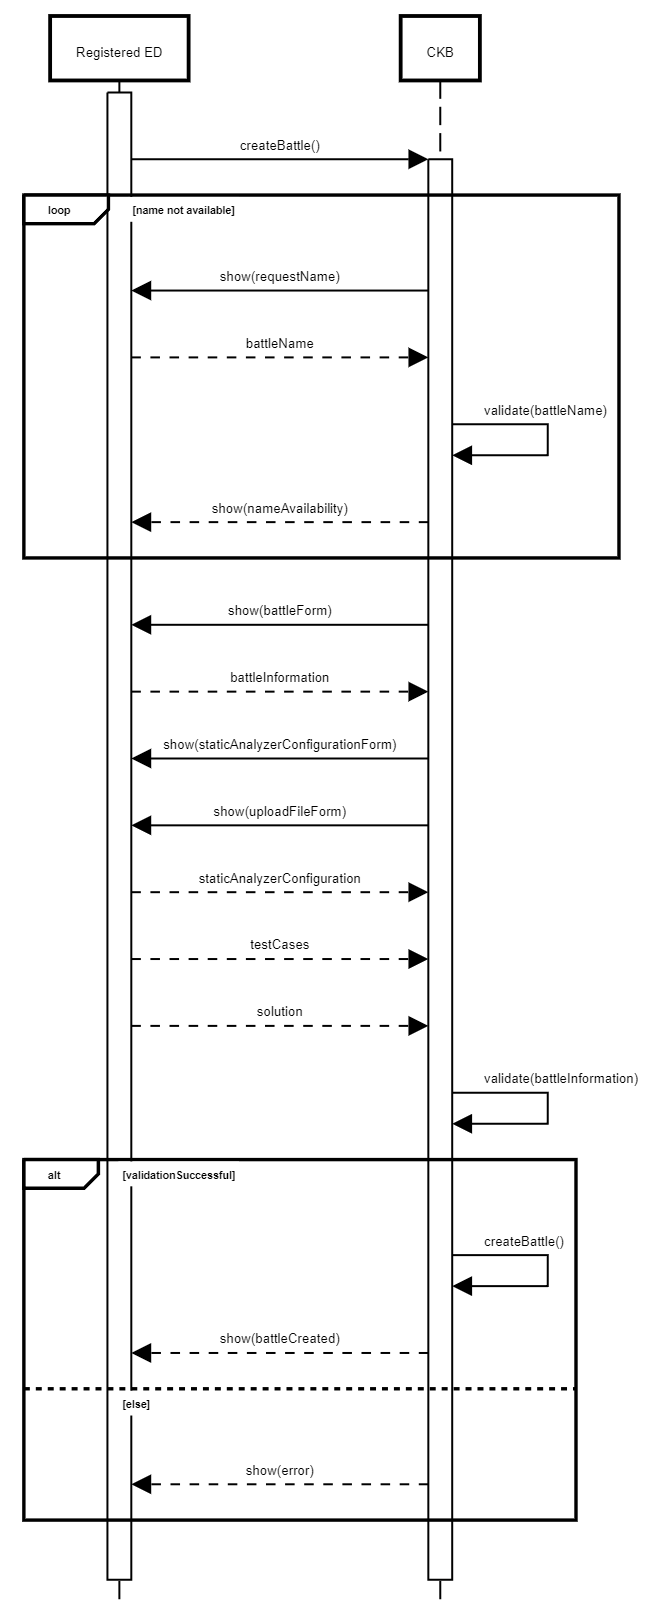
\includegraphics[width=\textwidth,height=\textheight,keepaspectratio]{Images/SequenceDiagrams/UC6.png}
        \caption{UC6 sequence diagram.}
        \label{fig: UC6_sequence_diagram}
    \end{center}
  \end{figure}
\end{center}

\subsubsection*{UC7: ED invites other EDs to a competition}
\begin{center}
  \begin{longtable}{l|p{0.75\linewidth}}
    \hline
    Actor & Registered ED \\
    \hline
    Entry conditions & The ED is already registered and logged in  \\
    & The ED is the creator or a collaborator of the competition \\
    & The ED is in the competition page \\
    \hline
    Event Flow & 1.\ ED clicks on the "Settings" button inside the competition\\
    & 2.\ ED scrolls down to the "Collaborators" section \\
    & 3.\ ED clicks on the "Invite" button \\
    & 4.\ CKB asks for the email or the username of the ED to invite \\
    & 5.\ ED inserts the email or the username \\
    & 6.\ CKB validates the information \\
    & 7.\ CKB sends an invitation email to the ED \\
    & 8.\ The invited ED clicks on the link received in the email \\
    & 9.\ CKB confirms the invitation  \\
    \hline
    Exit condition & The invited ED is a collaborator of the competition \\
    \hline
    Exceptions & 6.1 The email or the username is not valid \\
    & 8.1 The link is expired \\ \\
    & In all the cases the ED is notified with an error message \\
    \hline
    \caption{ED invites other EDs to a competition.}
    \label{tab: ED_invite_ED}
  \end{longtable}

  \begin{figure} [H]
    \begin{center}
        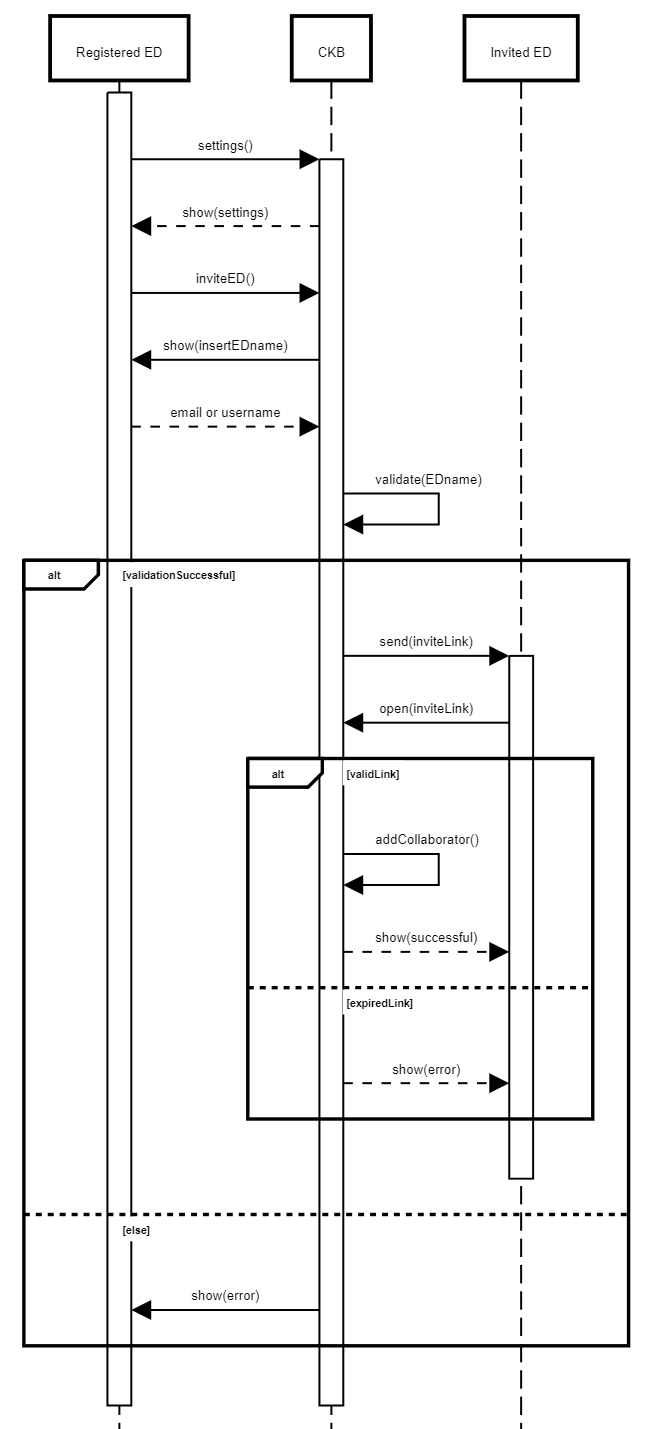
\includegraphics[width=\textwidth,height=\textheight,keepaspectratio]{Images/SequenceDiagrams/UC7.png}
        \caption{UC7 sequence diagram.}
        \label{fig: UC7_sequence_diagram}
    \end{center}
  \end{figure}
\end{center}

\subsubsection*{UC8: ED creates a new badge inside a competition}
\begin{center}
  \begin{longtable}{l|p{0.75\linewidth}}
    \hline
    Actor & Registered ED \\
    \hline
    Entry conditions & The ED is already registered and logged in  \\
    & The ED is the creator or a collaborator of the competition \\
    & The ED is in the competition page \\
    \hline
    Event Flow & 1.\ ED clicks on the "Settings" button inside the competition\\
    & 2.\ ED scrolls down to the "Badges" section \\
    & 3.\ ED clicks on the "Create new Badge" button \\
    & 4.\ CKB asks for the information (i.e. name, description) of the badge \\
    & 5.\ ED inserts the information \\
    & 6.\ CKB asks for the rules of the badge \\
    & 7.\ ED inserts the rules \\
    & 8.\ CKB validates the information \\
    & 9.\ CKB creates the badge \\
    \hline
    Exit condition &  The badge is added to the competition \\
    \hline
    Exceptions & 8.1 CKB isn’t able to validate the information \\ \\
    & The ED is notified with an error message \\
    \hline
    \caption{ED creates a badge inside a competition.}
    \label{tab: ED_create_badge}
  \end{longtable}

  \begin{figure} [H]
    \begin{center}
        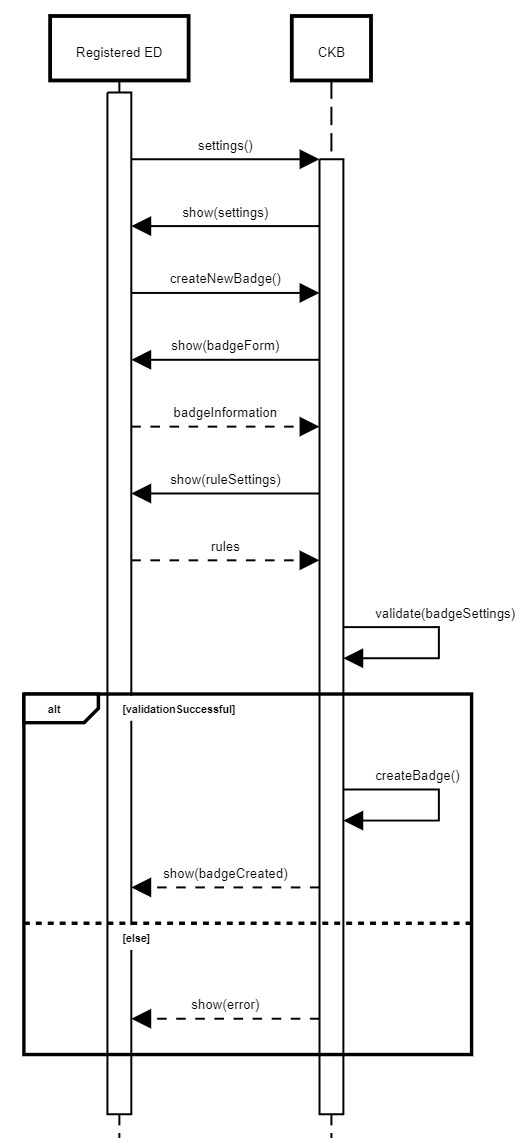
\includegraphics[width=\textwidth,height=\textheight,keepaspectratio]{Images/SequenceDiagrams/UC8.png}
        \caption{UC8 sequence diagram.}
        \label{fig: UC8_sequence_diagram}
    \end{center}
  \end{figure}
\end{center}

\subsubsection*{UC9: ST joins a battle}
\begin{center}
  \begin{longtable}{l|p{0.75\linewidth}}
    \hline
    Actor & Registered ST \\
    \hline
    Entry conditions & The ST is already registered  \\
    & The ST is enrolled in a competition \\
    & The ST is in the competition page \\
    \hline
    Event Flow & 1.\ CKB show the list of the battles inside of the competition \\
    & 2.\ The ST select the battle that wants to join \\
    & 3.\ CKB shows the information about the battle \\
    & 4.\ The ST clicks on the “Join” button \\
    & 5.\ CKB asks to create a new T or to join an existing one \\
    & Here there are two possibilities: \\
    & \quad \quad 6.1 The ST selects to create a new T \\
    & \quad \quad 6.1.1 CKB asks for the information about the team (i.e. name, number of members) \\
    & \quad \quad 6.1.2 The ST inserts the information \\
    & \quad \quad 6.1.3 CKB validate the information \\
    & \quad \quad 6.1.4 CKB asks for the name of the other STs to invite \\
    & \quad \quad 6.1.5 The ST inserts the name of the other STs \\
    & \quad \quad 6.1.6 CKB validate the information \\
    & \quad \quad 6.1.7 CKB sends the invites to the other STs \\
    & \quad \quad 6.1.8 CKB creates the T \\
    & 6.2 The ST selects to join an existing public T \\
    & \quad \quad 6.2.1 CKB shows the list of the public available Ts \\
    & \quad \quad 6.2.2 The ST selects the T \\
    & \quad \quad 6.2.3 CKB adds the ST to the T \\
    \hline
    Exit condition &  ST has joined the battle \\
    \hline
    Exceptions & 6.1.3 CKB isn’t able to validate the information \\
    & 6.1.6 CKB isn’t able to validate the information \\ \\
    & In all the cases the ST is notified with an error message \\

    \hline
    \caption{ST joins a battle.}
    \label{tab: ST_join_battle}
  \end{longtable}

  \begin{figure} [H]
    \begin{center}
        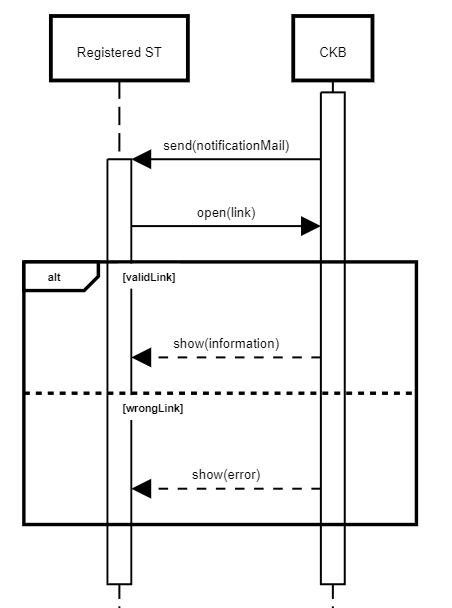
\includegraphics[width=0.65\textwidth,height=\textheight,keepaspectratio]{Images/SequenceDiagrams/UC9.png}
        \caption{UC9 sequence diagram.}
        \label{fig: UC9_sequence_diagram}
    \end{center}
  \end{figure}
\end{center}

\subsubsection*{UC10: ST visualizes the ranking of their T}
\begin{center}
  \begin{longtable}{l|p{0.75\linewidth}}
    \hline
    Actor & Registered ST \\
    \hline
    Entry conditions & The ST is already registered and logged in \\
    & The ST is enrolled in a competition \\
    & The ST is enrolled in a battle \\
    & The ST is in the competition page \\
    \hline
    Event Flow & 1.\ CKB shows the list of the battles in which the ST is enrolled \\
    & 2.\ The ST selects the battle \\
    & 3.\ The ST goes to the “Ranking” section \\
    & 4.\ CKB shows the ranking of the battle \\
    \hline
    Exit condition &  The ST visualize the ranking of their team \\
    \hline
    Exceptions & 2.1 There are no battles available \\ \\
    & In this case the ST visualizes a message that there are no battles available \\
    \hline
    \caption{ST visualizes the ranking of their T.}
    \label{tab: ST_visualize_ranking}
  \end{longtable}

  \begin{figure} [H]
    \begin{center}
        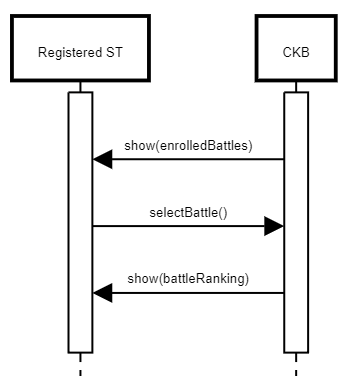
\includegraphics[width=0.35\textwidth,height=\textheight,keepaspectratio]{Images/SequenceDiagrams/UC10.png}
        \caption{UC10 sequence diagram.}
        \label{fig: UC10_sequence_diagram}
    \end{center}
  \end{figure}
\end{center}


\subsubsection*{UC11: ED manually evaluates the code}
\begin{center}
  \begin{longtable}{l|p{0.75\linewidth}}
    \hline
    Actor & Registered ED \\
    \hline
    Entry conditions & The ED is already registered  \\
    & The ED is the creator or a collaborator of the competition \\
    & The ED is in the battle page \\
    \hline
    Event Flow & 1.\ ED clicks on a T name \\
    & 2.\ CKB shows the information about the T \\
    & 3.\ ED clicks on the “Evaluate” button \\
    & 4.\ CKB shows the information about the last code submission \\
    & 5.\ ED navigates through the code \\
    & 6.\ ED assigns a score to the code \\
    & 7.\ CKB saves the score \\
    \hline
    Exit condition &  The score is saved \\
    \hline
    Exceptions & 4.1 The T didn't submit any code \\
    & 7.1 CKB isn’t able to save the score \\ \\
    & In the first case the ED visualize a message that there are no code submissions \\
    & In the other case the ED is notified with an error message \\
    \hline
    \caption{ED manually evaluates the code.}
    \label{tab: ED_evaluate_code}
  \end{longtable}

  \begin{figure} [H]
    \begin{center}
        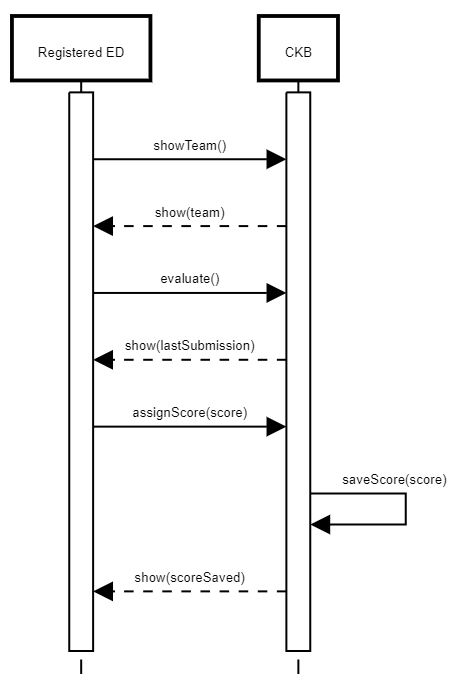
\includegraphics[width=0.60\textwidth,height=\textheight,keepaspectratio]{Images/SequenceDiagrams/UC11.png}
        \caption{UC11 sequence diagram.}
        \label{fig: UC11_sequence_diagram}
    \end{center}
  \end{figure}
\end{center}

\subsubsection*{UC12: ST accepts an invitation to join a T}
\begin{center}
  \begin{longtable}{l|p{0.75\linewidth}}
    \hline
    Actor & Registered ST \\
    \hline
    Entry conditions & The ST is already registered \\
    \hline
    Event Flow & 1.\ CKB sends an invitation email to join a team to the ST \\
    & 2.\ The ST clicks on the link received in the email \\
    & 3.\ CKB adds the ST to the T \\
    \hline
    Exit condition &  The ST joined the team \\
    \hline
    Exceptions & 2.1 The link is expired \\ \\
    & In this case the ST is notified with an error message \\
    \hline
    \caption{ST accepts an invitation to join a T.}
    \label{tab: ST_accepts_invitation}
  \end{longtable}

  \begin{figure} [H]
    \begin{center}
        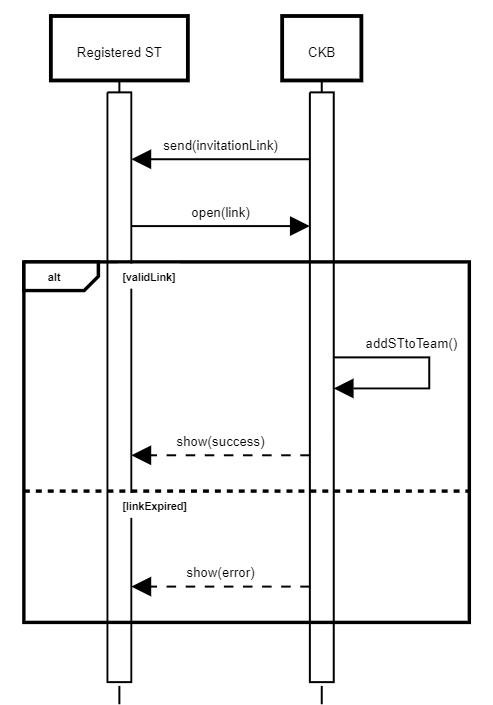
\includegraphics[width=0.50\textwidth,height=\textheight,keepaspectratio]{Images/SequenceDiagrams/UC12.png}
        \caption{UC12 sequence diagram.}
        \label{fig: UC12_sequence_diagram}
    \end{center}
  \end{figure}
\end{center}

\newpage

\section{Performance Requirements}
\label{s:Performance_requirements}%

\subsection*{Concurrent connections}
\label{ss:Concurrent_connections}%

Since the connections during the phases of the competitions will for sure be very high we need to ensure that the system can handle a big number of concurrent connections. Considering an average number of partecipant in a competition of 300 and an average number of battles per competition of 5, we can estimate that the number of concurrent connections will be around 2000. To ensure that multiple competition can be run at the same time we need to ensure that the system can handle at least 10000 concurrent connections.

\subsection*{Response time}
\label{ss:Response_time}%

The system should be able to respond to a request in less than 1 second. In particular the system should be able to respond to a request in less than 0.5 seconds for the most common requests (i.e. login, signup, create competition, create battle, join battle, join team, evaluate code, visualize ranking).

\subsection*{Scalability}
\label{ss:Scalability}%

The system should be able to scale to support more competitions and battles. In particular the system should be able to support at least 1000 competitions and 10000 battles.



\section{Design Constraints}
\label{s:Design_constraints}%

\subsection{Standard compliance}
\label{ss:Standard_compliance}%

The system should respect the laws about privacy and data protection of the country in which it is used. In particular for the use in Europe it should respect the GDPR. Morover the system should respect the data treatment for exchange with third party systems (i.e. GitHub).

\subsection{Hardware limitation}
\label{ss:Hardware_limitation}%

The system should be able to run on any device with a browser and an internet connection. The system should be able to run on any operating system.

\subsection{Any other constraint}
\label{ss:Any_other_constraint}%

There are no other constraints.

\section{Software System Attributes}
\label{s:Software_system_attributes}%

\subsection{Reliability}
\label{ss:Reliability}%

Since the system is not critical as the code from the student is uploaded on Github, it is not necessary to have a high reliability. It is reasonable to have a failure rate between 0.1\% and 1\% to ensure an high quality service. In any case the system should be able to recover the data and state in case of failure.

\subsection{Availability}
\label{ss:Availability}%

To ensure a good user experience and permit the ED to make changes to the competition and battles, the system should guarantee an availability of 99\%.


\subsection{Security}
\label{ss:Security}%

The system guarantees the security of the communication between the users and the server using the HTTPS protocol. The system should guarantee the security of the data stored in the database using encryption and access control. 

\subsection{Maintainability}
\label{ss:Maintainability}%

The system should be easy to maintain and update. The code should be well documented and the architecture should be well designed to allow the addition of new features and the correction of bugs.

\subsection{Portability}
\label{ss:Portability}%

The system does not have restriction on the operating system and the browser. The system should be developed as a web application with a responsive design to allow the use on different devices.